
\section{Magnetism III}

Name \rule{2.0in}{0.1pt}\hfill{}Section \rule{1.0in}{0.1pt}\hfill{}Date
\rule{1.0in}{0.1pt}

\textbf{Objectives}

To investigate:

\begin{itemize}
\item The effect of magnetic fields on moving charges. 
\item The effect of moving charges on magnets. 
\end{itemize}

\textbf{Apparatus} 

\begin{itemize} 
\item Bar magnet
\item Oscilloscope
\item Tangent galvanometer
\item Compass
\item Power supply
\end{itemize}

%\textbf{Introduction} 

%Where did this intro come from??? It has nothing to do with the lab!
%A charged object moving through a magnetic field experiences a force
%which is proportional to the magnitude of its charge and to its speed
%perpendicular to the field: $F = qvB_\perp$. Changing the number of
%magnetic field lines--the flux--through a coil of wire results in
%a current in the wire. The direction of this current is such that
%the magnetic field it produces opposes the change in the external
%field. Similarly, varying the current in one coil (the primary) produces
%a current in another nearby coil (the secondary). The current in the
%second coil, too, will flow in a direction that creates a magnetic
%field opposing that which is changing in the first coil. These relationships
%between changing fields and currents are known collectively as electromagnetic
%induction.



\textbf{Activity 1: Magnetic Forces on Moving Charges }

\begin{enumerate}
\item Turn on the oscilloscope by pressing the power button. Turn the TIME/DIV
knob completely counterclockwise. Adjust the INTEN (intensity) and
FOCUS knobs so that a small bright spot is formed on the oscilloscope
screen by the beam of electrons traveling toward you. Adjust the ILLUM
(illumination) knob so that the grid on the screen can be seen clearly.
Use the horizontal and vertical POSITION controls to center the spot
on the screen.
\item \textbf{Note}: An oscilloscope is built around the principle of the
cathode ray tube. It emits electrons from its back end. These are
accelerated by a series of electrodes and focused to strike a fluorescent
screen at its front. The result is a visible trace identifying voltage
as a function of time.
\item \textbf{Predictions}: What, if anything, will happen to the spot on
the screen if the north pole of a magnet is brought near the left
side of the oscilloscope? What will happen if you do the same with
the south pole? What about when each of the poles are brought near
to the top? {[}Please do not touch the oscilloscope with the magnet.{]} \vspace{30mm}

\item Bring the N-pole of a horizontal bar magnet near, but not touching,
the left side of the oscilloscope case at the height of the spot.
Record the direction of any deflection. Repeat with the S-pole.\vspace{20mm}

\item Bring the N-pole of a vertical bar magnet near, but not touching,
the top of the oscilloscope cast just above the spot. Record the direction
of any deflection. Repeat with the S-pole.\vspace{20mm}

\item Turn off the oscilloscope.
\item Did the directions of deflections meet your expectations? Explain. \vspace{15mm}

\end{enumerate}

\textbf{Activity 2: Moving Charges Effect on Magnets}

In this investigation we will use a device known as a tangent galvanometer to make
a qualitative study of the effect of current (moving charges) in a coil of wire
on a compass.
A sketch of the galvanometer is shown below.

\begin{center}
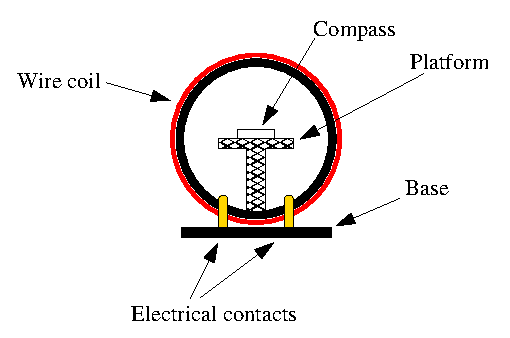
\includegraphics{tangent_galvanometer.eps}
\par
Figure 1. Tangent galvanometer and compass.
\end{center}

\begin{enumerate}

\item Connect the positive and negative electrodes on the power supply
to the two side screws on the tangent galvanometer.

\item With the power supply off, place the compass of the platform in the center of
the tangent galvanometer.
Align the compass and the plane of the wire coil of the galvanometer with
the  contacts of the galvanometer to the right.
Turn the power supply on and 
slowly turn up the voltage.
What do you observe?
Make a sketch to show the orientation of the compass and tangent
galvanometer with the voltage on and off.
\vspace{20mm}

\item Turn the voltage on the power supply to zero.
Rotate the entire setup (galvanometer, compass, wires) $180^\circ$
so it faces in the
opposite direction with the electric contacts now on the left side.
Make sure the plane of the wire coil and the compass are parallel.
Slowly turn the voltage back up. What do you observe?
Make another sketch to show the orientation of the compass and tangent
galvanometer with the voltage on and off.
\vspace{20mm}

\item The deflection of the compass when current flows in the tangent 
galvanometer implies the current creates a magnetic field.
From your observations can you tell the direction
of the magnetic field?  Explain.
%if
%there is a North pole to the magnetic field of the current in the coil?
%Is there a South pole? Explain using your observations from above.
\vspace{20mm}

\item Reverse the wires on the power supply to reverse the direction
of the current in the coil of the tangent galvanometer.
We will now repeat the observations from above.
With the voltage off, align the compass and the plane of the wire coil of the galvanometer with
the  contacts of the galvanometer to the right.
Slowly turn up the voltage.
What do you observe?
Make a sketch to show the orientation of the compass and tangent
galvanometer with the voltage on and off.
\vspace{20mm}

\item Rotate the entire setup (galvanometer, compass, wires) $180^\circ$
so it faces in the
opposite direction with the electric contacts now on the left side.
Make sure the plane of the wire coil and the compass are parallel.
Slowly turn the voltage back up. What do you observe?
 Make another sketch.
\vspace{20mm}

\item What happens to the magnetic field of the tangent galvanometer
when you reverse the direction of the current?

\end{enumerate}
